\graphicspath{{chapters/chapter7/imgs/}}

\chapter{Wyniki}\label{chapter:ch7}

W tym rozdziale przedstawione zostaną ostateczne wyniki przeprowadzonego eksperymentu, w tym: przedstawienie
demografii uczestników badania, dokonanie analizy ilościowej i jakościowej danych.

\section{Demografia}\label{section:ch7_1}

W badaniu wzięły udział 34 osoby, gdzie 14 uczestników wypełniło formularz A, a 20 osób formularz B.
Ogólny rozkład płci uczestników był stosunkowo wyrównany - w przypadku formularza A, 9 osób to kobiety, a 5 to
mężczyźni. Z kolei wśród wypełniających formularz B, 7 osób to kobiety, 12 to mężczyźni, a 1 osoba wybrała
opcję "Inna" w pytaniu o płeć. Te informacje można odczytać z tabeli \ref{tab1:ch7_1} i rysunku \ref{fig:ch7_demo1}.

\begin{table}[h!]
    \begin{center}
        \begin{tabular}{|l|r|r|}
            \hline
            Płeć      & Liczba osób & Procent całości \\
            \hline
            Kobieta   & 16          & 47,06\%         \\
            Mężczyzna & 17          & 50,00\%         \\
            Inne      & 1           & 2,94\%          \\
            \hline
        \end{tabular}
    \end{center}
    \caption{Uczestnicy badania ze względu na płeć}\label{tab1:ch7_1}
\end{table}

\begin{figure}[h!]
    \centering
    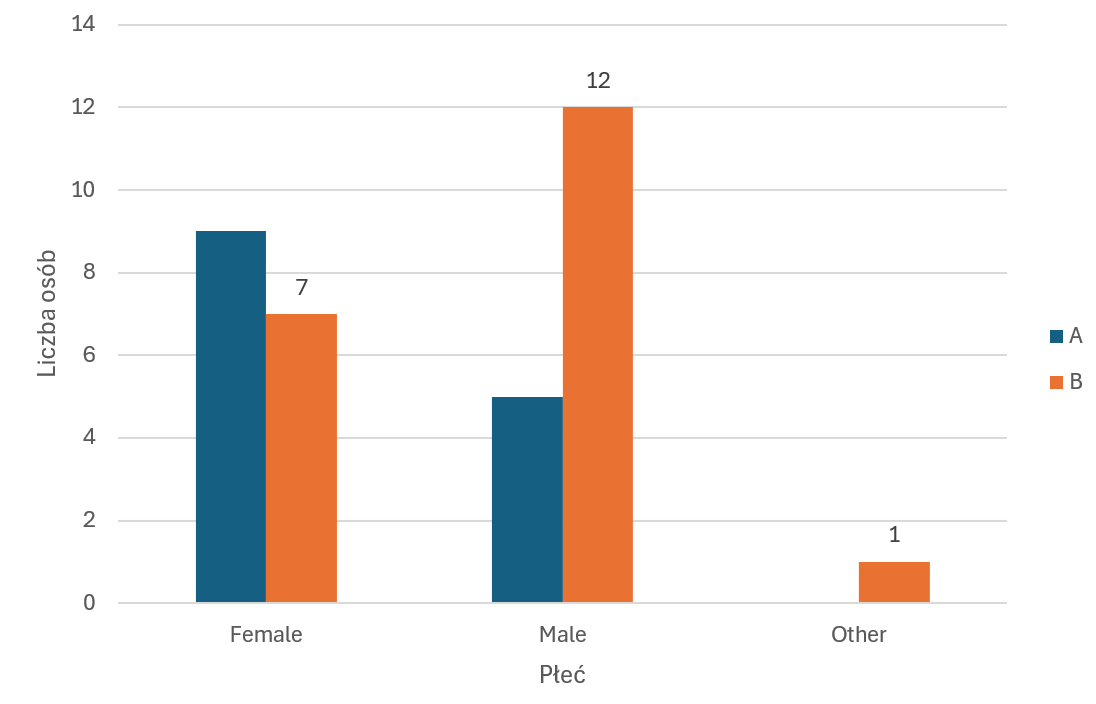
\includegraphics[width=0.9\textwidth]{demo1.png}
    \caption{Płeć uczestników badania z podziałem na formularz A i B}
    \label{fig:ch7_demo1}
\end{figure}

\newpage

Większość uczestników należała do grupy wiekowej 20-29 lat, co odzwierciedlają dane przedstawione w
tabeli \ref{tab1:ch7_2} i na rysunku \ref{fig:ch7_demo2} . Wśród wypełniających formularz A było 9 osób
w wieku 20-29 lat, a w przypadku formularza B - 11 osób. Uczestnicy reprezentowali jednak różne grupy
wiekowe, od nastolatków po osoby po 30. i 40. roku życia.

\begin{table}[h!]
    \begin{center}
        \begin{tabular}{|l|r|r|}
            \hline
            Przedział wiekowy & Liczba osób & Procent całości \\
            \hline
            15-19             & 4           & 11,76\%         \\
            20-24             & 12          & 35,29\%         \\
            25-29             & 8           & 23,53\%         \\
            30-34             & 6           & 17,65\%         \\
            35-39             & 3           & 8,82\%          \\
            40-45             & 1           & 2,94\%          \\
            \hline
        \end{tabular}
    \end{center}
    \caption{Uczestnicy badania ze względu na wiek}\label{tab1:ch7_2}
\end{table}

\begin{figure}[h!]
    \centering
    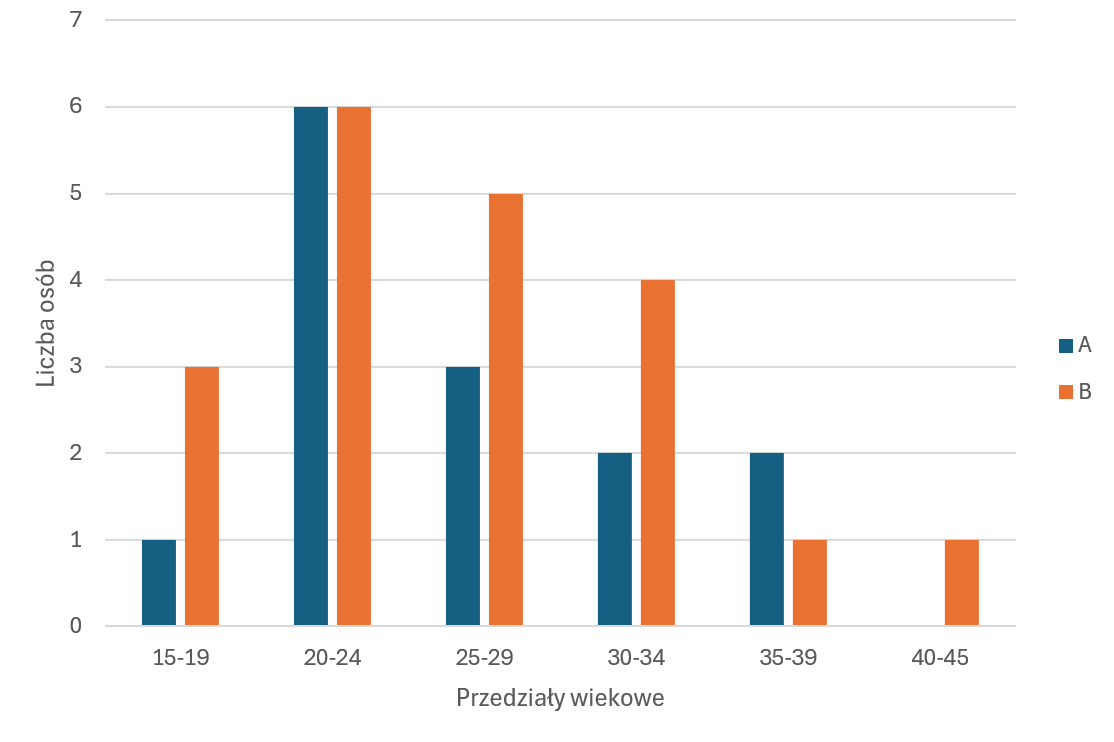
\includegraphics[width=0.9\textwidth]{demo2.png}
    \caption{Wiek uczestników badania z podziałem na formularz A i B}
    \label{fig:ch7_demo2}
\end{figure}

\newpage

Uczestnicy badania pochodzili z różnych kontynentów, jednak dominowali mieszkańcy Europy i Stanów
Zjednoczonych, co widać wyraźnie na rysunku \ref{fig:ch7_demo3} i w tabeli \ref{tab1:ch7_3} . Najwięcej
osób wypełniających formularz A pochodziło z Francji, Indii, Stanów Zjednoczonych i Wielkiej Brytanii. Z kolei w
przypadku formularza B, największe reprezentacje miały Stany Zjednoczone, Wielka Brytania i Niemcy.

\begin{table}[h!]
    \begin{center}
        \begin{tabular}{|l|r|r|}
            \hline
            Kraj pochodzenia  & Liczba osób & Procent całości \\
            \hline
            Antigua i Barbuda & 1           & 2,94\%          \\
            Argentyna         & 1           & 2,94\%          \\
            Chiny             & 1           & 2,94\%          \\
            Filipiny          & 1           & 2,94\%          \\
            Francja           & 3           & 8,82\%          \\
            Holandia          & 2           & 5,88\%          \\
            Indie             & 3           & 8,82\%          \\
            Niemcy            & 3           & 8,82\%          \\
            Nowa Zelandia     & 1           & 2,94\%          \\
            Polska            & 2           & 5,88\%          \\
            Portugalia        & 1           & 2,94\%          \\
            Rosja             & 1           & 2,94\%          \\
            Stany Zjednoczone & 7           & 20,59\%         \\
            Szwecja           & 1           & 2,94\%          \\
            Ukraina           & 1           & 2,94\%          \\
            Wielka Brytania   & 5           & 14,71\%         \\
            \hline
        \end{tabular}
    \end{center}
    \caption{Uczestnicy badania ze względu na kraj pochodzenia}\label{tab1:ch7_3}
\end{table}

\begin{figure}[h!]
    \centering
    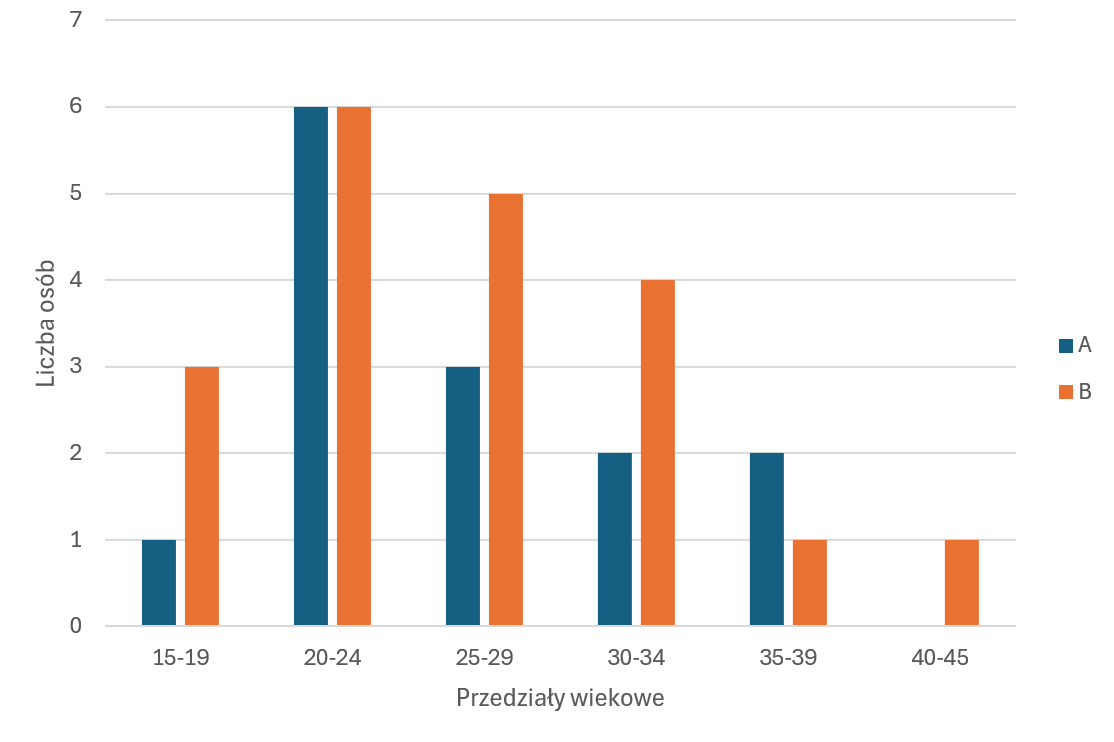
\includegraphics[width=0.9\textwidth]{demo3.png}
    \caption{Kraj pochodzenia uczestników badania z podziałem na formularz A i B}
    \label{fig:ch7_demo3}
\end{figure}

\newpage

Interesującym aspektem badania był wiek, w którym uczestnicy rozpoczęli przygodę z grami wideo. Jak
pokazują dane w tabeli \ref{tab1:ch7_4}  i na rysunku \ref{fig:ch7_demo4} , zdecydowana większość osób
zaczęła grać w wieku 7-12 lat. Pozostali zadeklarowali, że zaczęli grać przed 7. rokiem życia
lub w okresie nastoletnim (13-19 lat). Jedna osoba rozpoczęła przygodę z grami po dwudziestym roku życia.

\begin{table}[h!]
    \begin{center}
        \begin{tabular}{|l|r|r|}
            \hline
            Wiek rozpoczęcia grania w gry wideo & Liczba osób & Procent całości \\
            \hline
            <7                                  & 7           & 20,59\%         \\
            7-12                                & 19          & 55,88\%         \\
            13-15                               & 5           & 14,71\%         \\
            16-19                               & 2           & 5,88\%          \\
            20+                                 & 1           & 2,94\%          \\
            \hline
        \end{tabular}
    \end{center}
    \caption{Uczestnicy badania ze względu na wiek rozpoczęcia grania w gry wideo}\label{tab1:ch7_4}
\end{table}

\begin{figure}[h!]
    \centering
    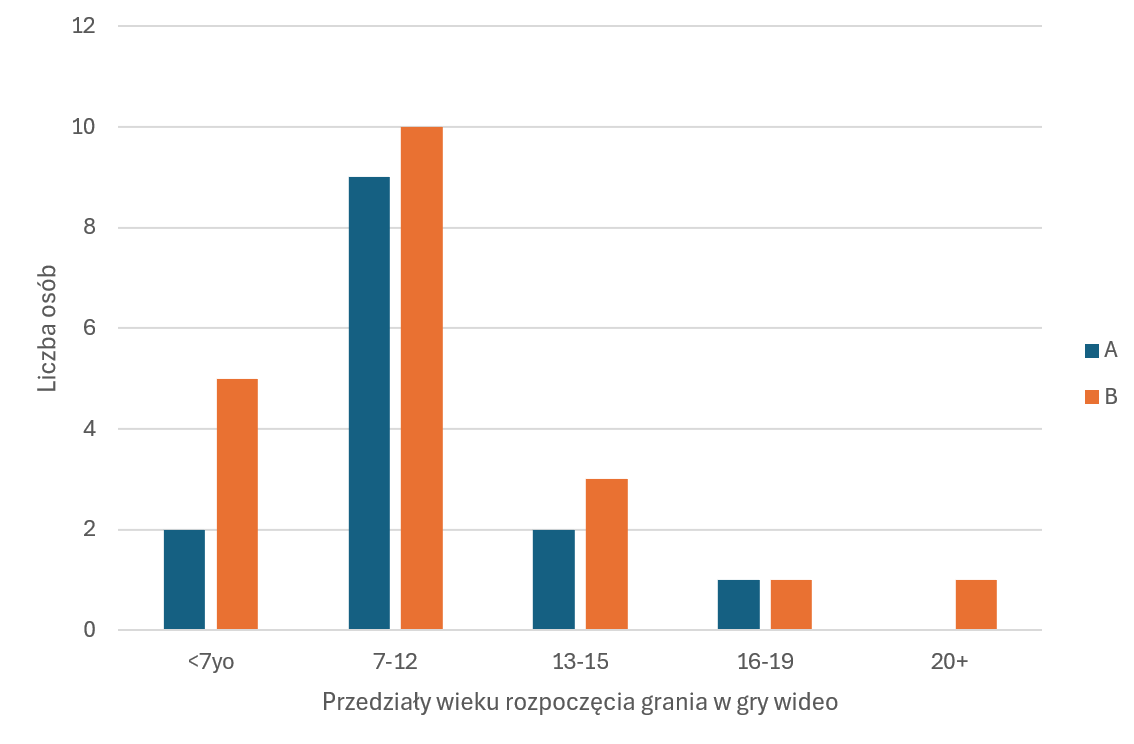
\includegraphics[width=0.9\textwidth]{demo4.png}
    \caption{Wiek rozpoczęcia grania w gry wideo przez uczestników badania z podziałem na formularz A i B}
    \label{fig:ch7_demo4}
\end{figure}

\newpage

Wreszcie, z danych przedstawionych na rysunku \ref{fig:ch7_demo5} i w tabeli \ref{tab1:ch7_5} wynika, że uczestnicy średnio nie spędzali
więcej niż 10 godzin tygodniowo na graniu. Najwięcej osób deklarowało granie przez mniej niż 5 godzin
tygodniowo lub w przedziale 5-10 godzin. Nieliczni przyznali, że grają ponad 20 godzin tygodniowo.

\begin{table}[h!]
    \begin{center}
        \begin{tabular}{|m{15em}|r|r|}
            \hline
            Średnia liczba godzin tygodniowo \newline przeznaczona na gry wideo & Liczba osób & Procent całości \\
            \hline
            <5h                                                                 & 16          & 47,06\%         \\
            5-10h                                                               & 10          & 29,41\%         \\
            10-15h                                                              & 2           & 5,88\%          \\
            15-20h                                                              & 2           & 5,88\%          \\
            >20h                                                                & 4           & 11,76\%         \\
            \hline
        \end{tabular}
    \end{center}
    \caption{Uczestnicy badania ze względu na średnią liczbę godzin tygodniowo przeznaczonych na gry wideo}\label{tab1:ch7_5}
\end{table}

\begin{figure}[h!]
    \centering
    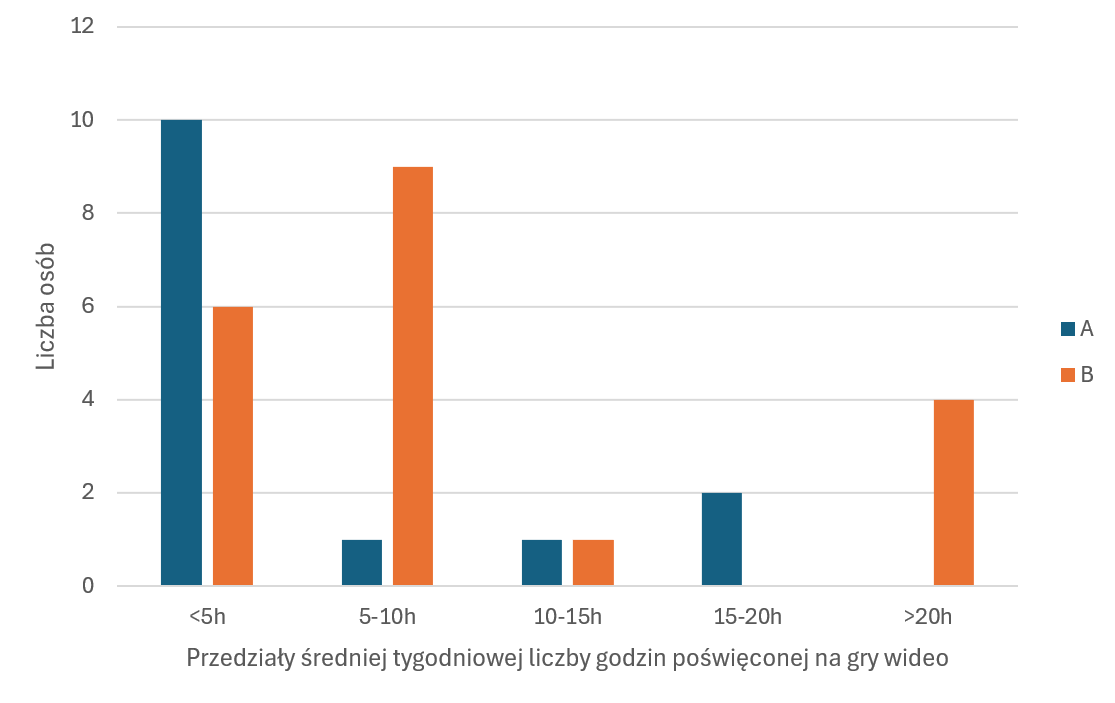
\includegraphics[width=0.9\textwidth]{demo5.png}
    \caption{Średnia liczba godzin tygodniowo przeznaczona na gry wideo przez uczestników badania z podziałem na formularz A i B}
    \label{fig:ch7_demo5}
\end{figure}

\newpage

\section{Analiza danych}\label{section:ch7_2}

W ramach analizy zebranych danych zdecydowano się na wykorzystanie testów statystycznych do porównania różnic między
odpowiedziami zarówno w ramach jednego formularza (pomiędzy wersją bez \gls{ai} i wersją z \gls{ai} dla tego samego uczestnika)
jak i pomiędzy formularzami (porównanie odpowiedzi dla odpowiednich wersji pomiędzy formularzem A i B). Poziom
istotności statystycznej, z którym porównane są wartości prawdopodobieństwa testowego, został przyjęty na poziomie 0,05.
Pytanie, które osiągnęło w dowolnej rubryce wartość \textit{p value} poniżej poziomu istotności statystycznej,
oznaczone zostało w tabeli poprzez znak "*" a powodująca to wartość \textit{p value} została pogrubiona.

Ze względu na niespełnienie założenia normalności rozkładu przez wiele pozycji w teście Shapiro-Wilka (co zostało
przedstawione w tabelach \ref{tab1:ch7_10} oraz \ref{tab1:ch7_11}), nie można było zastosować testu t-Studenta,
pomimo spełnienia założenia równości wariancji w teście Levene'a (co widać w tabeli \ref{tab1:ch7_12}). Zdecydowano
się więc na użycie nieparametrycznych testów statystycznych.

\newpage

\begin{table}[!h]
    \begin{center}
        \begin{tabular}{|m{10em}|m{5em}|m{5em}|m{5em}|m{5em}|}
            \hline
            Pytanie                                                                     & Wartość statystyki (non-\gls{ai}) & P-value (non-\gls{ai}) & Wartość statystyki (\gls{ai}) & P-value (\gls{ai}) \\
            \hline
            1. Tracę poczucie czasu                                                     & 0,911                             & 0,164                  & 0,900                         & 0,113              \\
            2. Byłem/-am \newline zainteresowany/-a fabułą gry                          & 0,923                             & 0,243                  & 0,881                         & 0,060              \\
            3. Czuję się inaczej\textbf{*}                                              & 0,855                             & \textbf{0,026}         & 0,886                         & 0,070              \\
            4. Czułem/-am, że mogę odkrywać różne rzeczy\textbf{*}                      & 0,755                             & \textbf{0,001}         & 0,837                         & \textbf{0,015}     \\
            5. Gra wydaje się prawdziwa\textbf{*}                                       & 0,841                             & \textbf{0,017}         & 0,903                         & 0,127              \\
            6. Byłem/-am \newline w pełni zajęty/-a grą\textbf{*}                       & 0,850                             & \textbf{0,023}         & 0,896                         & 0,100              \\
            7. Denerwuję się\textbf{*}                                                  & 0,900                             & 0,111                  & 0,814                         & \textbf{0,007}     \\
            8. Czas jakby stanął w miejscu lub się zatrzymał\textbf{*}                  & 0,834                             & \textbf{0,013}         & 0,837                         & \textbf{0,015}     \\
            9. Czuję się \newline rozkojarzony/-a\textbf{*}                             & 0,864                             & \textbf{0,034}         & 0,814                         & \textbf{0,007}     \\
            10. Byłem/-am głęboko \newline skoncentrowany/-a \newline na grze\textbf{*} & 0,914                             & 0,181                  & 0,848                         & \textbf{0,021}     \\
            11. Zmęczyłem/-am się\textbf{*}                                             & 0,867                             & \textbf{0,038}         & 0,909                         & 0,152              \\
            12. Granie wydaje się automatyczne\textbf{*}                                & 0,924                             & 0,253                  & 0,842                         & \textbf{0,017}     \\
            13. Moje myśli \newline biegną szybko\textbf{*}                             & 0,932                             & 0,326                  & 0,836                         & \textbf{0,014}     \\
            14. Podobało mi się\textbf{*}                                               & 0,878                             & 0,054                  & 0,875                         & \textbf{0,049}     \\
            15. Gram bez zastanawiania się jak grać\textbf{*}                           & 0,805                             & \textbf{0,006}         & 0,896                         & 0,100              \\
            16. Granie sprawia, \newline że czuję się spokojny/-a\textbf{*}             & 0,911                             & 0,164                  & 0,844                         & \textbf{0,018}     \\
            17. Gram dłużej \newline niż zamierzałem/-am\textbf{*}                      & 0,820                             & \textbf{0,009}         & 0,855                         & \textbf{0,026}     \\
            18. Naprawdę wczuwam się w grę                                              & 0,923                             & 0,246                  & 0,885                         & 0,069              \\
            19. Czuję, że nie mogę przestać grać\textbf{*}                              & 0,786                             & \textbf{0,003}         & 0,744                         & \textbf{0,001}     \\
            \hline
        \end{tabular}
    \end{center}
    \caption{Wyniki testu Shapiro-Wilka dla formularza A i obu wersji gier}\label{tab1:ch7_10}
\end{table}

\begin{table}[!h]
    \begin{center}
        \begin{tabular}{|m{10em}|m{5em}|m{5em}|m{5em}|m{5em}|}
            \hline
            Pytanie                                                                     & Wartość statystyki (non-\gls{ai}) & P-value (non-\gls{ai}) & Wartość statystyki (\gls{ai}) & P-value (\gls{ai}) \\
            \hline
            1. Tracę poczucie czasu\textbf{*}                                           & 0,892                             & \textbf{0,029}         & 0,836                         & \textbf{0,003}     \\
            2. Byłem/-am \newline zainteresowany/-a fabułą gry\textbf{*}                & 0,875                             & \textbf{0,014}         & 0,864                         & \textbf{0,009}     \\
            3. Czuję się inaczej\textbf{*}                                              & 0,793                             & \textbf{0,001}         & 0,882                         & \textbf{0,019}     \\
            4. Czułem/-am, że mogę odkrywać różne rzeczy\textbf{*}                      & 0,856                             & \textbf{0,007}         & 0,728                         & \textbf{0,000}     \\
            5. Gra wydaje się prawdziwa\textbf{*}                                       & 0,827                             & \textbf{0,002}         & 0,867                         & \textbf{0,010}     \\
            6. Byłem/-am \newline w pełni zajęty/-a grą\textbf{*}                       & 0,854                             & \textbf{0,006}         & 0,842                         & \textbf{0,004}     \\
            7. Denerwuję się\textbf{*}                                                  & 0,792                             & \textbf{0,001}         & 0,847                         & \textbf{0,005}     \\
            8. Czas jakby stanął w miejscu lub się zatrzymał\textbf{*}                  & 0,827                             & \textbf{0,002}         & 0,864                         & \textbf{0,009}     \\
            9. Czuję się \newline rozkojarzony/-a\textbf{*}                             & 0,865                             & \textbf{0,010}         & 0,917                         & \textbf{0,088}     \\
            10. Byłem/-am głęboko \newline skoncentrowany/-a \newline na grze\textbf{*} & 0,883                             & \textbf{0,020}         & 0,792                         & \textbf{0,001}     \\
            11. Zmęczyłem/-am się\textbf{*}                                             & 0,860                             & \textbf{0,008}         & 0,902                         & \textbf{0,045}     \\
            12. Granie wydaje się automatyczne\textbf{*}                                & 0,789                             & \textbf{0,001}         & 0,893                         & \textbf{0,031}     \\
            14. Podobało mi się\textbf{*}                                               & 0,890                             & \textbf{0,000}         & 0,865                         & \textbf{0,010}     \\
            15. Gram bez zastanawiania się jak grać\textbf{*}                           & 0,746                             & \textbf{0,006}         & 0,896                         & \textbf{0,034}     \\
            16. Granie sprawia, \newline że czuję się spokojny/-a\textbf{*}             & 0,851                             & \textbf{0,006}         & 0,825                         & \textbf{0,002}     \\
            17. Gram dłużej \newline niż zamierzałem/-am\textbf{*}                      & 0,840                             & \textbf{0,004}         & 0,860                         & \textbf{0,008}     \\
            18. Naprawdę wczuwam się w grę\textbf{*}                                    & 0,876                             & \textbf{0,015}         & 0,875                         & \textbf{0,015}     \\
            19. Czuję, że nie mogę przestać grać\textbf{*}                              & 0,850                             & \textbf{0,005}         & 0,882                         & \textbf{0,019}     \\
            \hline
        \end{tabular}
    \end{center}
    \caption{Wyniki testu Shapiro-Wilka dla formularza B i obu wersji gier}\label{tab1:ch7_11}
\end{table}

\begin{table}[!h]
    \begin{center}
        \begin{tabular}{|m{10em}|m{5em}|m{5em}|m{5em}|m{5em}|}
            \hline
            Pytanie                                                           & Wartość statystyki (non-\gls{ai}) & P-value (non-\gls{ai}) & Wartość statystyki (\gls{ai}) & P-value (\gls{ai}) \\
            \hline
            1. Tracę poczucie czasu                                           & 0,613                             & 0,439                  & 0,313                         & 0,580              \\
            2. Byłem/-am \newline zainteresowany/-a fabułą gry                & 0,121                             & 0,730                  & 1,395                         & 0,246              \\
            3. Czuję się inaczej                                              & 1,202                             & 0,281                  & 0,141                         & 0,710              \\
            4. Czułem/-am, że mogę odkrywać różne rzeczy                      & 3,149                             & 0,086                  & 0,004                         & 0,949              \\
            5. Gra wydaje się prawdziwa                                       & 2,329                             & 0,137                  & 0,054                         & 0,818              \\
            6. Byłem/-am \newline w pełni zajęty/-a grą                       & 0,070                             & 0,793                  & 0,281                         & 0,600              \\
            7. Denerwuję się                                                  & 0,388                             & 0,538                  & 0,168                         & 0,685              \\
            8. Czas jakby stanął w miejscu lub się zatrzymał                  & 1,340                             & 0,256                  & 0,121                         & 0,731              \\
            9. Czuję się \newline rozkojarzony/-a                             & 0,980                             & 0,330                  & 0,000                         & 1,000              \\
            10. Byłem/-am głęboko \newline skoncentrowany/-a \newline na grze & 0,009                             & 0,926                  & 1,252                         & 0,272              \\
            11. Zmęczyłem/-am się                                             & 0,003                             & 0,956                  & 0,059                         & 0,810              \\
            12. Granie wydaje się automatyczne                                & 0,408                             & 0,528                  & 2,819                         & 0,103              \\
            13. Moje myśli \newline biegną szybko                             & 0,693                             & 0,411                  & 0,604                         & 0,443              \\
            14. Podobało mi się                                               & 0,163                             & 0,689                  & 2,875                         & 0,100              \\
            15. Gram bez zastanawiania się jak grać                           & 1,740                             & 0,196                  & 0,227                         & 0,637              \\
            16. Granie sprawia, \newline że czuję się spokojny/-a             & 0,000                             & 1,000                  & 1,026                         & 0,319              \\
            17. Gram dłużej \newline niż zamierzałem/-am                      & 1,355                             & 0,253                  & 0,320                         & 0,576              \\
            18. Naprawdę wczuwam się w grę                                    & 0,254                             & 0,617                  & 0,399                         & 0,532              \\
            19. Czuję, że nie mogę przestać grać                              & 0,508                             & 0,481                  & 0,640                         & 0,430              \\
            \hline
        \end{tabular}
    \end{center}
    \caption{Wyniki testu Levene'a porównującego wariancję pomiędzy formularzem A i B odpowiednio dla wersji gier bez \gls{ai} i z \gls{ai}}\label{tab1:ch7_12}
\end{table}

\clearpage

W celu porównania różnic pomiędzy wersją bez \gls{ai} i wersją z \gls{ai} wewnątrz formularzy A i B, wykorzystano test
nieparametryczny Wilcoxona z zaztosowaną korektą na ciągłość. Analizując wyniki dla formularza A, uzyskano istotne statystycznie różnice dla
pozycji "Granie wydaje się automatyczne" (p = 0,031), "Gra wydaje się prawdziwa" (p = 0,012) oraz "Czułem/-am, że
mogę odkrywać różne rzeczy" (p = 0,003). W przypadku formularza B, istotne różnice odnotowano dla pozycji
"Czułem/-am, że mogę odkrywać różne rzeczy" (p = 0,002), "Granie wydaje się automatyczne" (p = 0,024),
"Gram bez zastanawiania się jak grać" (p = 0,008) oraz "Gram dłużej niż zamierzałem/-am" (p = 0,030). Pozycje 1 i 7
były stosunkowo blisko progu.

\begin{table}[!h]
    \begin{center}
        \begin{tabular}{|m{12em}|m{5em}|m{4em}|m{5em}|m{4em}|}
            \hline
            Pytanie                                                           & Wartość statystyki (A) & P-value (A)    & Wartość statystyki (B) & P-value (B)    \\
            \hline
            1. Tracę poczucie czasu                                           & 8                      & 0,152          & 12,5                   & 0,067          \\
            2. Byłem/-am \newline zainteresowany/-a fabułą gry                & 6                      & 0,783          & 27,5                   & 0,197          \\
            3. Czuję się inaczej                                              & 4                      & 0,408          & 21                     & 0,533          \\
            4. Czułem/-am, że mogę odkrywać różne rzeczy\textbf{*}            & 1,5                    & \textbf{0,003} & 0                      & \textbf{0,002} \\
            5. Gra wydaje się prawdziwa\textbf{*}                             & 0                      & \textbf{0,012} & 19,5                   & 0,759          \\
            6. Byłem/-am \newline w pełni zajęty/-a grą                       & 6,5                    & 0,890          & 41,5                   & 0,803          \\
            7. Denerwuję się                                                  & 10,5                   & 0,605          & 7                      & 0,066          \\
            8. Czas jakby stanął w miejscu lub się zatrzymał                  & 11                     & 0,665          & 25                     & 0,266          \\
            9. Czuję się \newline rozkojarzony/-a                             & 1,5                    & 0,586          & 22,5                   & 0,193          \\
            10. Byłem/-am głęboko \newline skoncentrowany/-a \newline na grze & 6,5                    & 0,890          & 22,5                   & 0,636          \\
            11. Zmęczyłem/-am się                                             & 18                     & 0,624          & 28                     & 0,684          \\
            12. Granie wydaje się automatyczne\textbf{*}                      & 1                      & \textbf{0,031} & 5                      & \textbf{0,024} \\
            13. Moje myśli \newline biegną szybko                             & 0                      & 0,089          & 20                     & 0,437          \\
            14. Podobało mi się                                               & 9                      & 0,830          & 20                     & 0,236          \\
            15. Gram bez zastanawiania się jak grać\textbf{*}                 & 5                      & 0,077          & 3                      & \textbf{0,008} \\
            16. Granie sprawia, \newline że czuję się spokojny/-a             & 14,5                   & 0,669          & 34,5                   & 0,745          \\
            17. Gram dłużej \newline niż zamierzałem/-am\textbf{*}            & 6                      & 0,766          & 6                      & \textbf{0,030} \\
            18. Naprawdę wczuwam się w grę                                    & 10,5                   & 1,000          & 16                     & 0,243          \\
            19. Czuję, że nie mogę przestać grać                              & 2                      & 0,773          & 21                     & 0,524          \\
            \hline
        \end{tabular}
    \end{center}
    \caption{Wyniki testu Wilcoxona porównującego zmianę ocen pytań wewnątrz formularza A i B}\label{tab1:ch7_13}
\end{table}

\newpage

Wykonano porównanie odpowiednich wariantów gry (bez \gls{ai} i z \gls{ai}) pomiędzy formularzem A i B za pomocą testu
Manna-Whitneya z zastosowaną korektą na ciągłość. Stwierdzono istotne statystycznie różnice dla pozycji "Czułem/-am, że mogę odkrywać różne rzeczy"
zarówno w wersji bez \gls{ai} (p = 0,004), jak i w wersji z \gls{ai} (p = 0,004). Różnice pomiędzy formularzami
A i B dla wersji bez \gls{ai} zaobserwowano również dla pozycji "Gra wydaje się prawdziwa" (p = 0,023) oraz "Granie wydaje
się automatyczne" (p = 0,044). W przypadku wersji z użyciem \gls{ai}, pomiędzy formularzami A i B odnotowano różnice dla
pozycji "Tracę poczucie czasu" (p = 0,025), "Granie sprawia, że czuję się spokojny/-a" (p = 0,015) oraz "Gram
dłużej niż zamierzałem/-am" (p = 0,048). Pozycje 9 i 19 były stosunkowo blisko progu.

\begin{table}[h!]
    \begin{center}
        \begin{tabular}{|m{10em}|m{5em}|m{5em}|m{5em}|m{5em}|}
            \hline
            Pytanie                                                           & Wartość statystyki (non-\gls{ai}) & P-value (non-\gls{ai}) & Wartość statystyki (\gls{ai}) & P-value (\gls{ai}) \\
            \hline
            1. Tracę poczucie czasu\textbf{*}                                 & 133                               & 0,816                  & 77                            & \textbf{0,025}     \\
            2. Byłem/-am \newline zainteresowany/-a fabułą gry                & 118                               & 0,440                  & 100                           & 0,154              \\
            3. Czuję się inaczej                                              & 121                               & 0,503                  & 123,5                         & 0,567              \\
            4. Czułem/-am, że mogę odkrywać różne rzeczy\textbf{*}            & 58,5                              & \textbf{0,004}         & 221                           & \textbf{0,004}     \\
            5. Gra wydaje się prawdziwa\textbf{*}                             & 77                                & \textbf{0,023}         & 133,5                         & 0,829              \\
            6. Byłem/-am \newline w pełni zajęty/-a grą                       & 112                               & 0,323                  & 101                           & 0,167              \\
            7. Denerwuję się                                                  & 154,5                             & 0,611                  & 138,5                         & 0,971              \\
            8. Czas jakby stanął w miejscu lub się zatrzymał                  & 106                               & 0,227                  & 95                            & 0,110              \\
            9. Czuję się \newline rozkojarzony/-a                             & 115,5                             & 0,389                  & 85                            & 0,051              \\
            10. Byłem/-am głęboko \newline skoncentrowany/-a \newline na grze & 106,5                             & 0,237                  & 107                           & 0,242              \\
            11. Zmęczyłem/-am się                                             & 133,5                             & 0,829                  & 159                           & 0,504              \\
            12. Granie wydaje się automatyczne\textbf{*}                      & 84,5                              & \textbf{0,044}         & 88                            & 0,064              \\
            13. Moje myśli \newline biegną szybko                             & 120,5                             & 0,493                  & 92,5                          & 0,090              \\
            14. Podobało mi się                                               & 123                               & 0,552                  & 106                           & 0,221              \\
            15. Gram bez zastanawiania się jak grać                           & 107                               & 0,220                  & 113,5                         & 0,352              \\
            16. Granie sprawia, \newline że czuję się spokojny/-a\textbf{*}   & 97,5                              & 0,129                  & 72,5                          & \textbf{0,015}     \\
            17. Gram dłużej \newline niż zamierzałem/-am\textbf{*}            & 129,5                             & 0,719                  & 84,5                          & \textbf{0,048}     \\
            18. Naprawdę wczuwam się w grę                                    & 119,5                             & 0,474                  & 105,5                         & 0,222              \\
            19. Czuję, że nie mogę przestać grać                              & 102                               & 0,175                  & 87,5                          & 0,062              \\
            \hline
        \end{tabular}
    \end{center}
    \caption{Wyniki testu Manna-Whitneya porównującego skalę ocen wersji gier bez \gls{ai} i z \gls{ai} pomiędzy formularzem A i B}\label{tab1:ch7_14}
\end{table}

\newpage

Test Wilcoxona wykazał istotne różnice pomiędzy wersjami gry bez \gls{ai} i z \gls{ai} w obrębie formularzy A i B
dla pozycji związanej z odkrywaniem świata gry oraz pozycji związanej z automatycznością. Przejście z
wersji bez \gls{ai} na wersję z \gls{ai} w ramach formularza A wykazało istotną różnicę dotyczącą postrzegania
prawdziwości świata gry. W przypadku formularza B "zabranie" \gls{ai} związane było z istotnymi zmianami
w obrębie postrzegania czasu poświęconego na grę oraz gry bez zastanawiania się.

Analiza testem Manna-Whitneya ujawniła różnice pomiędzy formularzami A i B dla niektórych pozycji, przy
czym część różnic była widoczna tylko w wersji bez \gls{ai}, a część tylko w wersji z \gls{ai}. Sugeruje to, że formuła
eksperymentu (ogrywanie dwóch wersji jedna po drugiej) miała wpływ na postrzeganie niektórych aspektów
rozgrywki. Może to oznaczać, że pierwsze doświadczenie jest de facto oceną bazową gry a drugie wypełnienie
kwestionariusza ujawnia wyraźne różnice po dodaniu lub zabraniu \gls{ai}.

Dla niektórych pozycji (np. 1, 7, 9, 19) wyniki były bliskie progu istotności statystycznej, co
sugeruje możliwość uzyskania dodatkowych różnic przy większej liczbie uczestników badania.

\vspace{10pt}

Oto najczęściej pojawiające się motywy w ramach pytań otwartych dla wersji bez \gls{ai}:

\begin{enumerate}
    \item Odczucie braku realizmu i statyczności interakcji z \gls{npc}.
    \item Przeciętne zainteresowanie rozmową z \gls{npc}, gdyż gracze nie czuli się naprawdę zaangażowani.
    \item Niezadowolenie z ograniczonej ilości informacji otrzymywanych od \gls{npc}.
    \item Duży podział jeśli chodzi o ostateczną przyjemność interakcji: część graczy
          narzekała na brak interakcji a dla części predefiniowane dialogi były na tyle dobre,
          że nie przeszkadzało im to.
\end{enumerate}

Natomiast dla wersji z \gls{ai} wystąpiły najczęściej takie motywy:

\begin{enumerate}
    \item Większe zainteresowanie rozmową z \gls{npc} i możliwością zadawania dowolnych pytań.
    \item Odczucie większego realizmu i lepszej immersji podczas interakcji.
    \item Zadowolenie z możliwości uzyskania większej ilości informacji od \gls{npc}.
    \item Frustracja spowodowana czasem odpowiedzi \gls{npc} lub ich niekompletnymi odpowiedziami.
    \item Rozproszenie uwagi od głównej rozgrywki z powodu zbyt wielu opcji konwersacji.
    \item Większość zadeklarowała duże poczucie przyjemności z interakcji z \gls{npc}.
\end{enumerate}

Dokładne odpowiedzi na pytania otwarte zostały zawarte w ramach dodatku \ref{appendix:C}.